\documentclass[border=6pt]{standalone}
% Shared draw.io-matching colours and node styles for the thesis flowcharts.
\usepackage{tikz}
\usetikzlibrary{shapes.geometric, arrows.meta, positioning, calc}

% Keep words whole inside boxes (no ugly mid-word hyphenation)
\hyphenpenalty=10000\exhyphenpenalty=10000\tolerance=2000

% draw.io standard palette (fill + stroke)
\definecolor{dioBlueF}{HTML}{DAE8FC}\definecolor{dioBlueS}{HTML}{6C8EBF}
\definecolor{dioOrangeF}{HTML}{FFE6CC}\definecolor{dioOrangeS}{HTML}{D79B00}
\definecolor{dioGrayF}{HTML}{F5F5F5}\definecolor{dioGrayS}{HTML}{666666}
\definecolor{dioGreenF}{HTML}{D5E8D4}\definecolor{dioGreenS}{HTML}{82B366}
\definecolor{dioPurpleF}{HTML}{E1D5E7}\definecolor{dioPurpleS}{HTML}{9673A6}

\tikzset{
  >={Stealth[length=2.4mm]},
  fnode/.style={rounded corners=5pt, draw, line width=0.8pt,
    minimum width=2.7cm, minimum height=1.15cm, align=center,
    font=\small, text width=2.5cm, inner sep=2pt},
  blue/.style ={fnode, fill=dioBlueF,   draw=dioBlueS},
  orange/.style={fnode, fill=dioOrangeF, draw=dioOrangeS},
  gray/.style ={fnode, fill=dioGrayF,   draw=dioGrayS},
  green/.style={fnode, fill=dioGreenF,  draw=dioGreenS},
  purple/.style={fnode, fill=dioPurpleF, draw=dioPurpleS},
  decision/.style={diamond, draw, line width=0.8pt, aspect=1.7,
    align=center, font=\small, text width=1.9cm, inner sep=0pt,
    fill=dioGrayF, draw=dioGrayS, minimum width=3cm, minimum height=2.3cm},
  bdecision/.style={decision, fill=dioBlueF, draw=dioBlueS},
  flow/.style={->, line width=0.8pt, draw=black!75},
  elabel/.style={font=\footnotesize, inner sep=1.5pt, fill=white},
}

\begin{document}
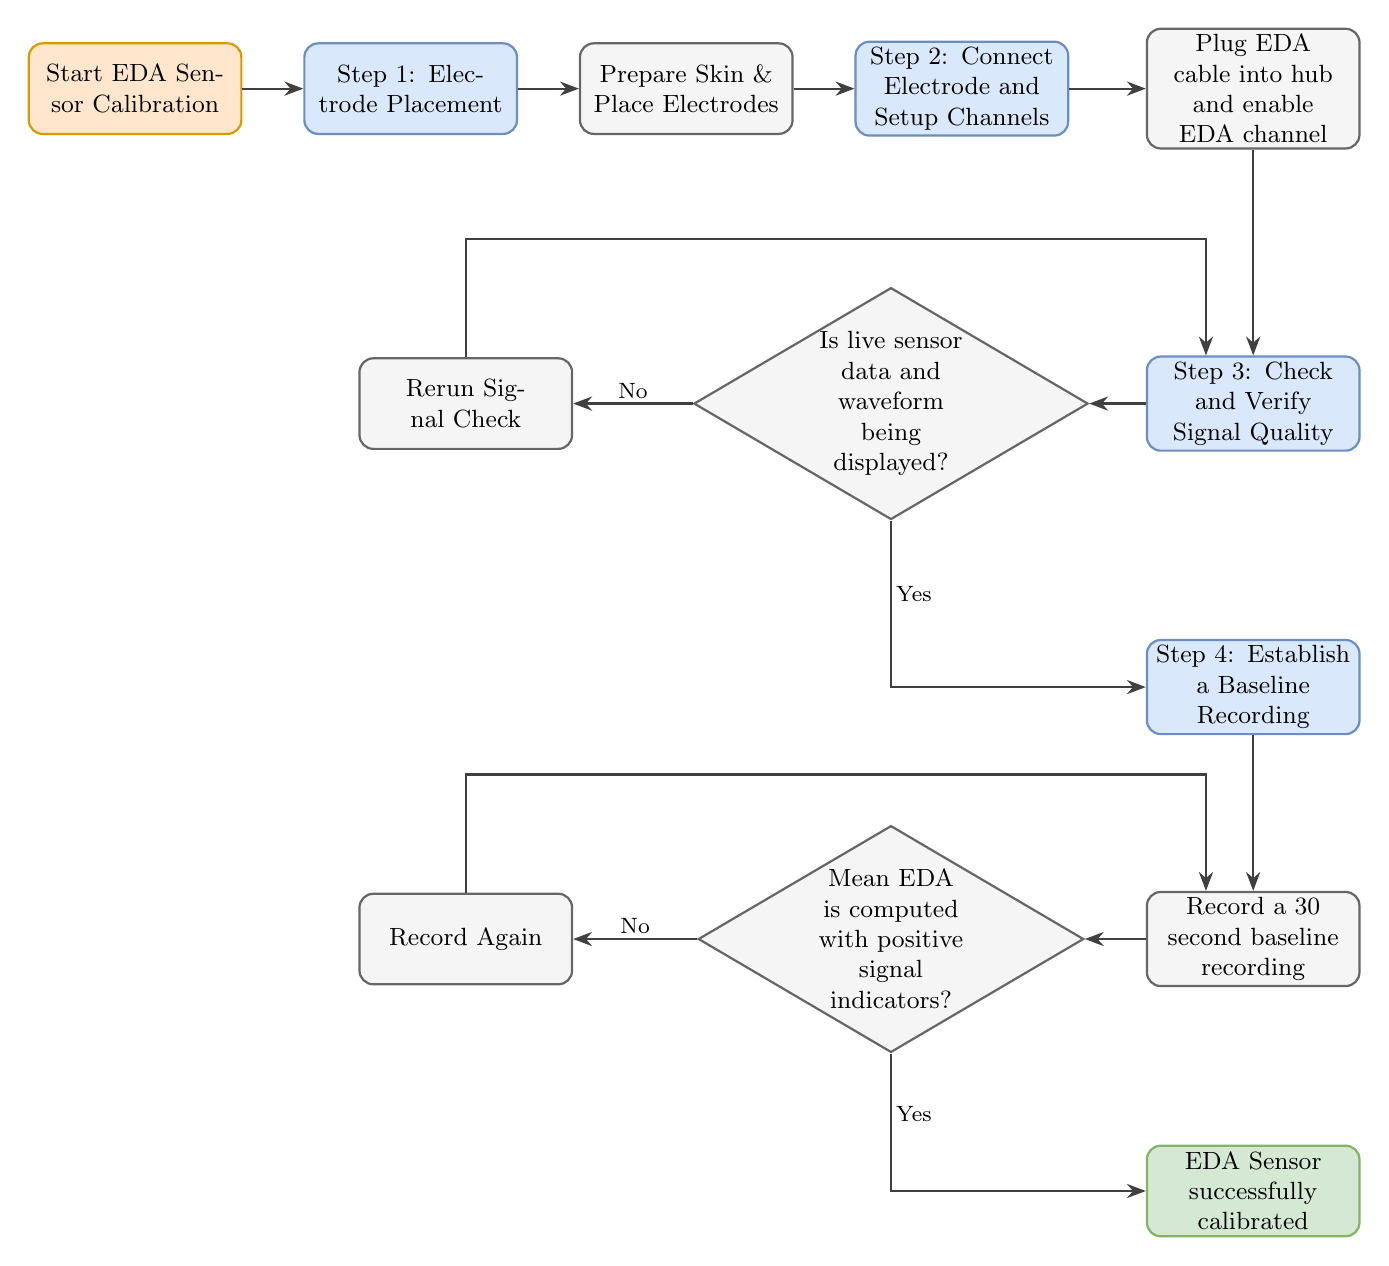
\begin{tikzpicture}

  % ---- Top row: electrode placement and channel setup ----------------------
  \node[orange] (start) at (0,0)     {Start EDA Sensor Calibration};
  \node[blue]   (step1) at (3.5,0)   {Step 1: Electrode Placement};
  \node[gray]   (skin)  at (7,0)     {Prepare Skin \& Place Electrodes};
  \node[blue]   (step2) at (10.5,0)  {Step 2: Connect Electrode and Setup Channels};
  \node[gray]   (plug)  at (14.2,0)  {Plug EDA cable into hub and enable EDA channel};

  \draw[flow] (start) -- (step1);
  \draw[flow] (step1) -- (skin);
  \draw[flow] (skin)  -- (step2);
  \draw[flow] (step2) -- (plug);

  % ---- Signal check loop ---------------------------------------------------
  \node[blue]    (step3) at (14.2,-4)  {Step 3: Check and Verify Signal Quality};
  \node[decision](live)  at (9.6,-4)   {Is live sensor data and waveform being displayed?};
  \node[gray]    (rerun) at (4.2,-4)   {Rerun Signal Check};

  \draw[flow] (plug) -- (step3);
  \draw[flow] (step3) -- node[elabel,above]{} (live);
  \draw[flow] (live) -- node[elabel,above]{No} (rerun);
  % rerun loops back into step 3 from above
  \draw[flow] (rerun.north) -- ++(0,1.5) -| ($(step3.north)+(-0.6,0)$);

  % ---- Baseline recording loop ----------------------------------------------
  \node[blue]    (step4) at (14.2,-7.6)  {Step 4: Establish a Baseline Recording};
  \draw[flow] (live.south) |- node[elabel,pos=0.22,right]{Yes} ($(step4.west)+(-0.4,0)$) -- (step4.west);

  \node[gray]    (rec30) at (14.2,-10.8) {Record a 30 second baseline recording};
  \node[decision](meaneda) at (9.6,-10.8){Mean EDA is computed with positive signal indicators?};
  \node[gray]    (again) at (4.2,-10.8)  {Record Again};
  \node[green]   (done)  at (14.2,-14)   {EDA Sensor successfully calibrated};

  \draw[flow] (step4) -- (rec30);
  \draw[flow] (rec30) -- (meaneda);
  \draw[flow] (meaneda) -- node[elabel,above]{No} (again);
  % record-again loops back into the 30-second recording from above
  \draw[flow] (again.north) -- ++(0,1.5) -| ($(rec30.north)+(-0.6,0)$);
  \draw[flow] (meaneda.south) |- node[elabel,pos=0.22,right]{Yes} ($(done.west)+(-0.4,0)$) -- (done.west);

\end{tikzpicture}
\end{document}
